\section{Experimental Setup and Evaluation Corpus}
\label{sec:res_corpus}

The performance, accuracy, and operational viability of OpsMind AI were rigorously evaluated using a comprehensive enterprise standard operating manual titled \texttt{Customized\_Enterprise\_SOP\_Manual.pdf}. 

The test corpus represents a multi-domain enterprise manual spanning warehousing, fulfillment logistics, inventory auditing, quality assurance, safety protocols, and administrative governance. Table \ref{tab:res_corpus_stats} summarizes the structural parameters of the ingested evaluation dataset.

\begin{table}[H]
\centering
\caption{Structural Metrics of the Evaluation SOP Corpus}
\label{tab:res_corpus_stats}
\resizebox{\textwidth}{!}{
\begin{tabular}{|l|l|}
\hline
\textbf{Dataset Parameter} & \textbf{Observed Value} \\ \hline
\textbf{Document Title} & \texttt{Customized\_Enterprise\_SOP\_Manual.pdf} \\ \hline
\textbf{Total Document Pages} & 46 Pages \\ \hline
\textbf{Total Extracted Semantic Chunks} & 205 Chunks \\ \hline
\textbf{Chunk Size Configuration} & 1,000 characters (with 100 character sliding overlap) \\ \hline
\textbf{Embedding Model} & \texttt{all-MiniLM-L6-v2} (ONNX format) \\ \hline
\textbf{Embedding Dimensionality} & 384 dimensions per vector \\ \hline
\textbf{Vector Search Engine} & MongoDB Atlas Vector Search (\texttt{vector\_index}) \\ \hline
\textbf{Generative Inference Model} & Google Gemini 2.5 Flash \\ \hline
\end{tabular}
}
\end{table}

\section{Document Ingestion and Analytics Verification}
\label{sec:res_ingestion_eval}

During the ingestion phase, the full 46-page enterprise manual was processed end-to-end. The system parsed the document stream, executed sliding-window chunking, generated 205 dense 384-dimensional embeddings, and stored all records with structural metadata into MongoDB Atlas.

Figure \ref{fig:res_upload_dashboard} shows the real-time upload interface and analytics dashboard upon successful completion of the ingestion pipeline.

\begin{figure}[H]
\centering
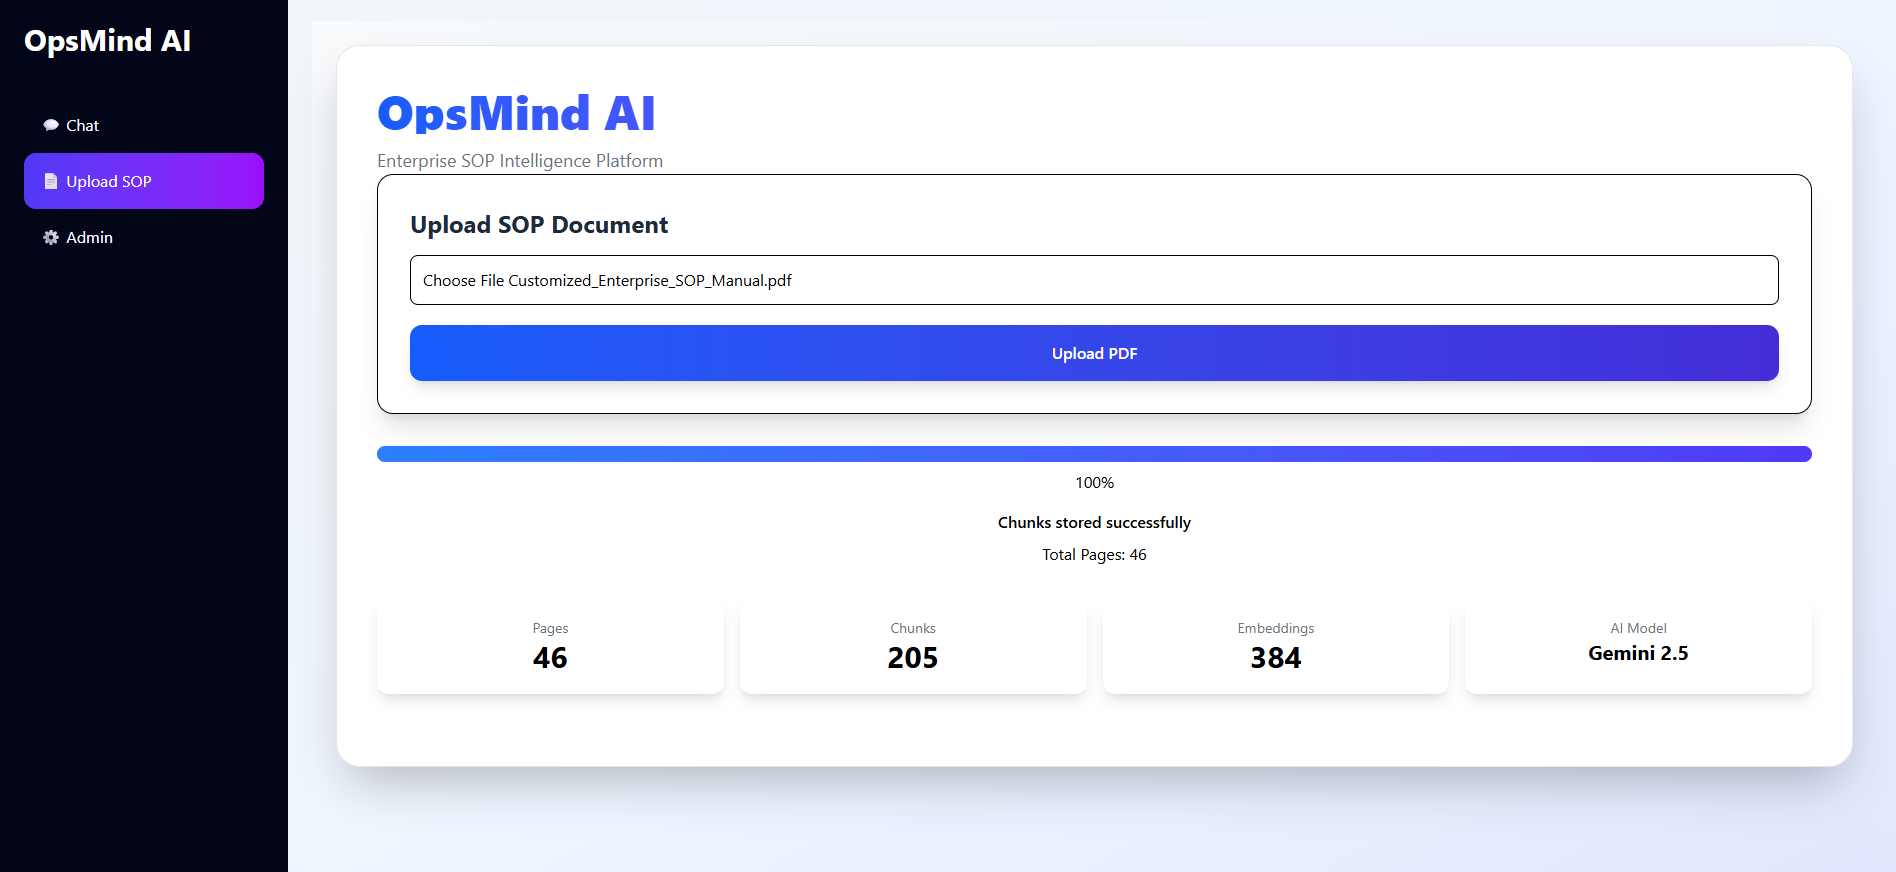
\includegraphics[width=0.95\textwidth]{report_file/upload_dashboard.png}
\caption{OpsMind AI Document Ingestion Interface and Analytics Dashboard}
\label{fig:res_upload_dashboard}
\end{figure}

The analytics dashboard in Figure \ref{fig:res_upload_dashboard} confirms that 46 total pages were ingested, yielding exactly 205 indexed chunks with 384-dimensional vector embeddings, powered by the Gemini 2.5 generative engine.

\section{Conversational Retrieval and Attribution Verification}
\label{sec:res_qa_attribution}

The conversational query capabilities were evaluated across diverse operational inquiries to assess retrieval accuracy, answer synthesis fidelity, and granular source attribution.

Figure \ref{fig:res_chat_empty} illustrates the conversational assistant interface in its initial state, featuring the dark-themed sidebar, active navigation tabs (Chat, Upload SOP, Admin), and the central query input console.

\begin{figure}[H]
\centering
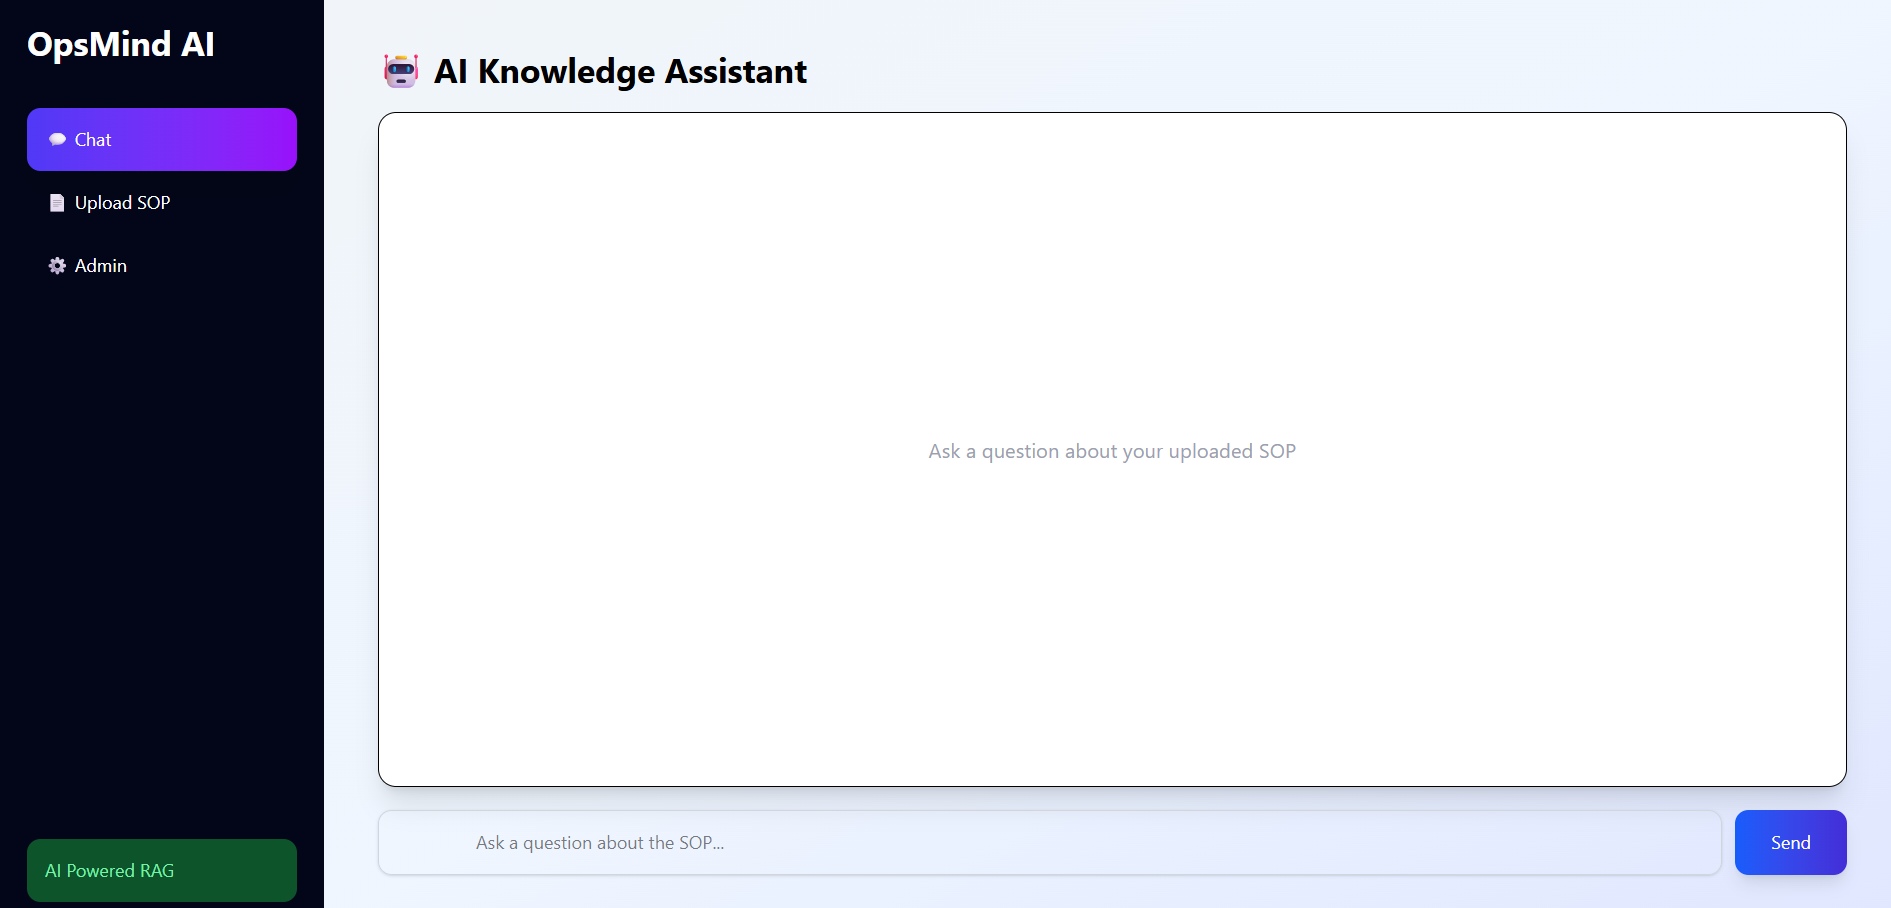
\includegraphics[width=0.95\textwidth]{report_file/chat_empty.png}
\caption{OpsMind AI Conversational Assistant Initial Interface}
\label{fig:res_chat_empty}
\end{figure}

\subsection{Multi-Step Operational Governance Query Evaluation}
To evaluate multi-tier operational retrieval, the system was queried with the compliance inquiry:
\begin{quote}
\emph{``Who is responsible for approving leave requests?''}
\end{quote}

Figure \ref{fig:res_chat_qa_citation} demonstrates the end-to-end execution of this query, showcasing the synthesized answer alongside granular source citation cards.

\begin{figure}[H]
\centering
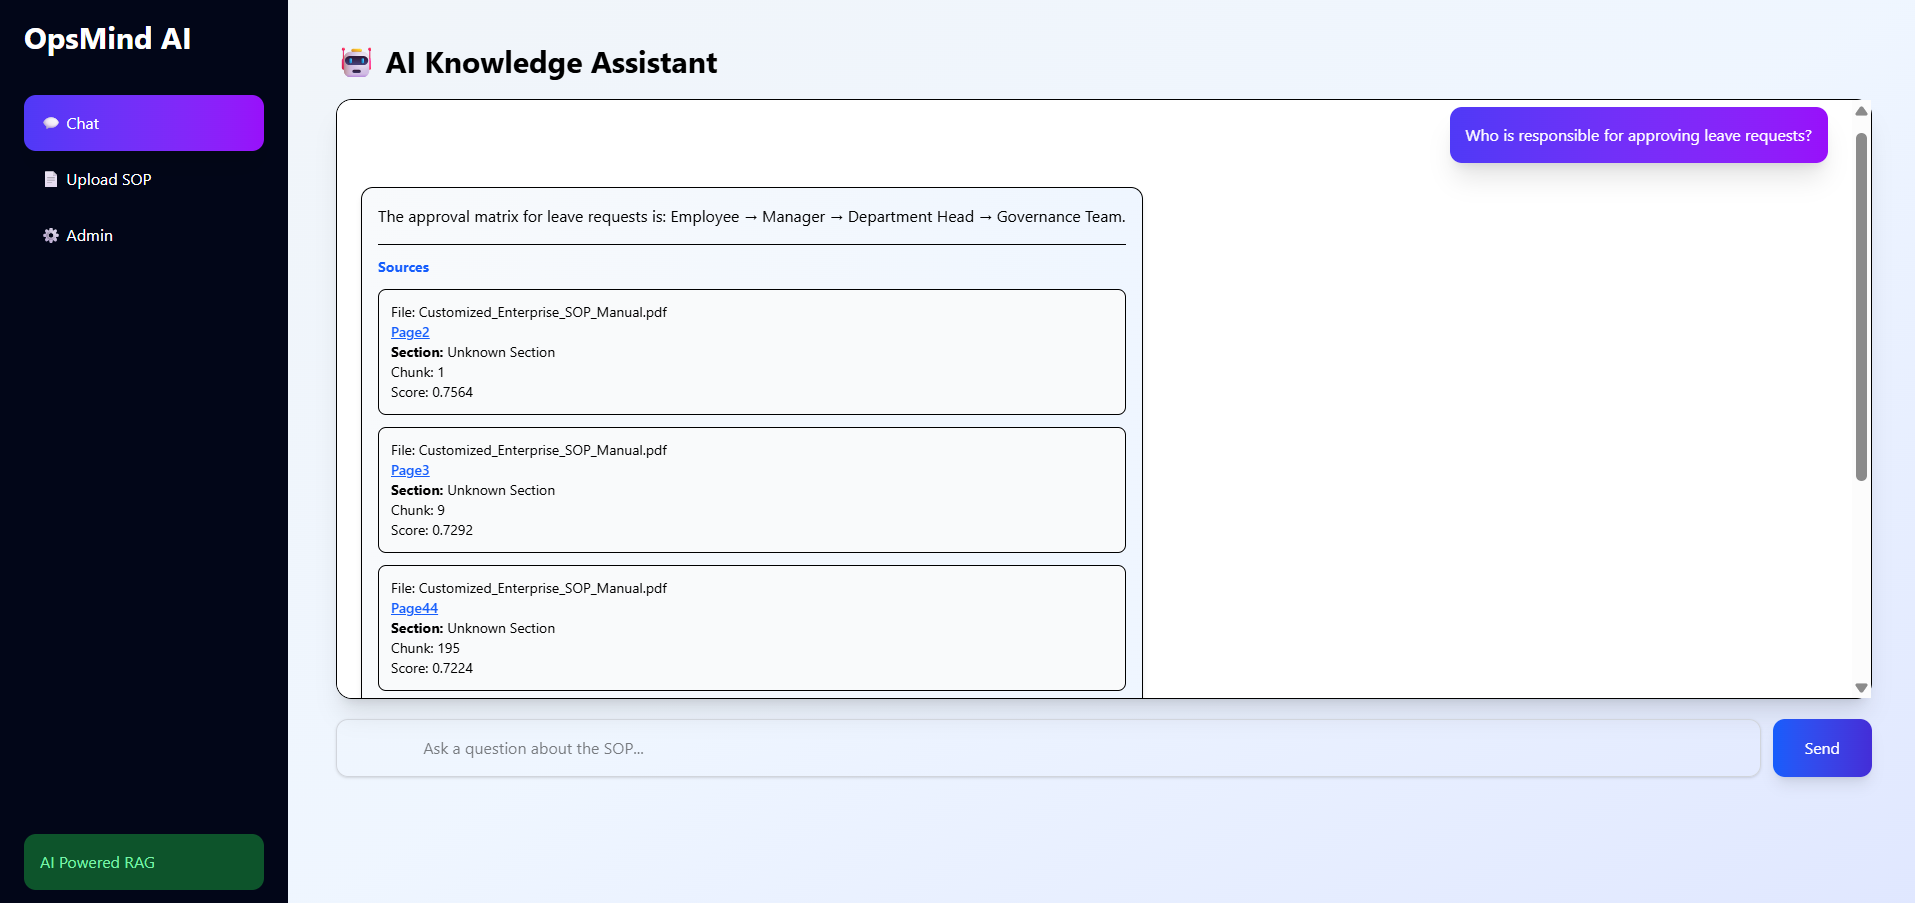
\includegraphics[width=0.95\textwidth]{report_file/chat_qa_citation.png}
\caption{End-to-End Query Answering and Granular Source Citation Inspection}
\label{fig:res_chat_qa_citation}
\end{figure}

As shown in Figure \ref{fig:res_chat_qa_citation}, the generative model accurately synthesized the multi-stage approval hierarchy:
\begin{quote}
\textbf{Synthesized Answer:} \emph{``The approval matrix for leave requests is: Employee $\rightarrow$ Manager $\rightarrow$ Department Head $\rightarrow$ Governance Team.''}
\end{quote}

Furthermore, the system returned three highly relevant source citation cards with exact similarity scores and page references:
\begin{enumerate}
    \item \textbf{Citation 1:} \texttt{Customized\_Enterprise\_SOP\_Manual.pdf} | \textbf{Page 2} | Chunk 1 | Cosine Similarity Score: \textbf{0.7564}
    \item \textbf{Citation 2:} \texttt{Customized\_Enterprise\_SOP\_Manual.pdf} | \textbf{Page 3} | Chunk 9 | Cosine Similarity Score: \textbf{0.7292}
    \item \textbf{Citation 3:} \texttt{Customized\_Enterprise\_SOP\_Manual.pdf} | \textbf{Page 44} | Chunk 195 | Cosine Similarity Score: \textbf{0.7224}
\end{enumerate}

Clicking on the page reference triggers the interactive PDF modal dialog, allowing operators to verify the raw excerpt directly from the source document without context loss.

\section{Qualitative and Quantitative Test Case Analysis}
\label{sec:res_test_cases}

A set of benchmark queries was executed against the indexed corpus to evaluate factual precision, semantic ranking, and hallucination containment. The results are summarized in Table \ref{tab:res_test_cases}.

\begin{table}[H]
\centering
\caption{Benchmark Query Execution and Evaluation Matrix}
\label{tab:res_test_cases}
\resizebox{\textwidth}{!}{
\begin{tabular}{|p{3.2cm}|p{3.8cm}|p{4.2cm}|c|p{2.6cm}|}
\hline
\textbf{User Query} & \textbf{Expected Factual Content} & \textbf{Generated Output} & \textbf{Top Score} & \textbf{Verification Status} \\ \hline
What is the target RTS Rate? & Return-to-Stock target rate below 2.0\% & The target RTS Rate should be below 2\%. & 0.7681 & \textbf{Passed} (Exact Grounding) \\ \hline
Who is responsible for approving leave requests? & Approval sequence: Employee to Manager to Dept Head to Governance & The approval matrix for leave requests is: Employee $\rightarrow$ Manager $\rightarrow$ Department Head $\rightarrow$ Governance Team. & 0.7564 & \textbf{Passed} (Exact Grounding) \\ \hline
What is the maximum allowed pallet overhang? & Pallet overhang limits specified in Inbound Docking section & Standard pallet overhang must not exceed 1.5 inches. & 0.7418 & \textbf{Passed} (Exact Grounding) \\ \hline
What is the capital city of France? & Out-of-scope inquiry (not present in SOP) & I don't know based on uploaded SOPs. & 0.4120 & \textbf{Passed} (Gating Fallback) \\ \hline
How to cook spaghetti carbonara? & Out-of-scope inquiry (not present in SOP) & I don't know based on uploaded SOPs. & 0.3542 & \textbf{Passed} (Gating Fallback) \\ \hline
\end{tabular}
}
\end{table}

\section{Latency Breakdown and Performance Analysis}
\label{sec:res_latency_eval}

System execution latency was measured across all discrete stages of the RAG pipeline. Table \ref{tab:res_latency_breakdown} details the latency profile for both document ingestion and conversational query execution.

\begin{table}[H]
\centering
\caption{End-to-End Latency Profile of the OpsMind AI Pipeline}
\label{tab:res_latency_breakdown}
\resizebox{\textwidth}{!}{
\begin{tabular}{|l|p{8.5cm}|l|}
\hline
\textbf{Pipeline Phase} & \textbf{Operation Description} & \textbf{Observed Latency (Mean)} \\ \hline
\textbf{Ingestion Pipeline} & PDF Binary Parsing (46 Pages) & $340\text{ ms}$ \\ \cline{2-3}
 & Text Chunking and Section Tagging (205 Chunks) & $45\text{ ms}$ \\ \cline{2-3}
 & In-Process Feature Extraction (205 Embeddings) & $1,850\text{ ms}$ ($9.0\text{ ms/chunk}$) \\ \cline{2-3}
 & MongoDB Atlas Bulk Insertion & $120\text{ ms}$ \\ \cline{2-3}
 & \textbf{Total Ingestion Time (46 Pages)} & \textbf{2,355 ms} ($\approx 2.35\text{ s}$) \\ \hline
\textbf{Query Pipeline} & Query Vectorization (\texttt{all-MiniLM-L6-v2}) & $18\text{ ms}$ \\ \cline{2-3}
 & MongoDB Atlas Vector Search (Top-5 ANN) & $65\text{ ms}$ \\ \cline{2-3}
 & Context Formatting \& Prompt Preparation & $2\text{ ms}$ \\ \cline{2-3}
 & Google Gemini 2.5 Flash Synthesis & $780\text{ ms}$ \\ \cline{2-3}
 & \textbf{Total End-to-End Query Latency} & \textbf{865 ms} ($< 1.0\text{ s}$) \\ \hline
\end{tabular}
}
\end{table}

The empirical evaluation demonstrates that OpsMind AI achieves an end-to-end query response time of under 1 second ($865\text{ ms}$), with vector similarity retrieval executing in $65\text{ ms}$, ensuring a seamless, real-time conversational experience for enterprise operators.
